\subsection{Interval estimate}
\label{sec:etas-interval}


Deciding on a ``best'' single-value estimate of arrival time is exceedingly difficult given the amount of uncertainty involved. The best approach above is to use a small quantile, but this then results in a large expected wait time given catching the bus (top-right of \cref{fig:eta_headway_results}). An alternative approach is to provide \emph{two} estimates---a lower and upper bound---that is to say, a \emph{prediction interval}. Such an interval should be both \emph{reliable} and \emph{useful} for commuters. Reliability means that, if one arrives by the \emph{lower estimate}, there is only a small probability of missing the bus. Additionally, the bus should also have a low chance of arriving after the \emph{upper estimate}, for example when using the prediction to decide which bus to catch to get to a destination on time (more of this in \cref{sec:etas-journey-planning}). Usefulness corresponds to the width and expected wait time: these should both be minimised where possible, so for example if a bus is 5~minutes away, providing a 30~minute interval should only be done if there is very good reason to do so. If the stop before is a layover, the time range could very well be that large since, as we discussed in \cref{cha:prediction}, drivers do not always wait, so there is a trade-off between reliability and usefulness.







In this section, we consider symmetric prediction intervals of the form $(\Teta_{\alpha/2}, \Teta_{1-\alpha/2})$ where $\alpha \in (0,1)$ gives a $100(1-\alpha)$\% interval. It should be noted that although these intervals are symmetric in probability, they are most often asymmetric on the arrival time scale since, particularly when the bus is near and the distribution is right-skewed, as shown in \cref{fig:eta_dist_skew}. In contrast, a \Kf{} implementation assumes Gaussian errors, so the interval would be symmetric around the mean, which will often lead to incorrect intervals (potentially even an \gls{eta} below zero).


\begin{knitrout}\small
\definecolor{shadecolor}{rgb}{0.969, 0.969, 0.969}\color{fgcolor}\begin{figure}

{\centering 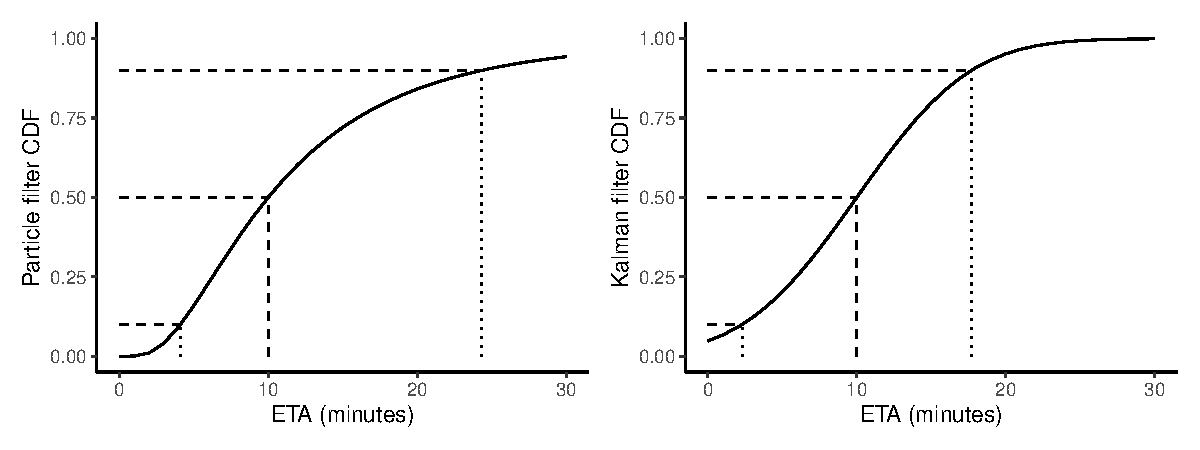
\includegraphics[width=\textwidth]{figure/eta_dist_skew-1} 

}

\caption[Symmetry of arrival time intervals]{Symmetry of arrival time intervals. Symmetric intervals on the probabilty scale map to asymmetric under the particle filter (left), and symmetric intervals under the Kalman filter (right).}\label{fig:eta_dist_skew}
\end{figure}


\end{knitrout}


\begin{knitrout}\small
\definecolor{shadecolor}{rgb}{0.969, 0.969, 0.969}\color{fgcolor}\begin{figure}

{\centering 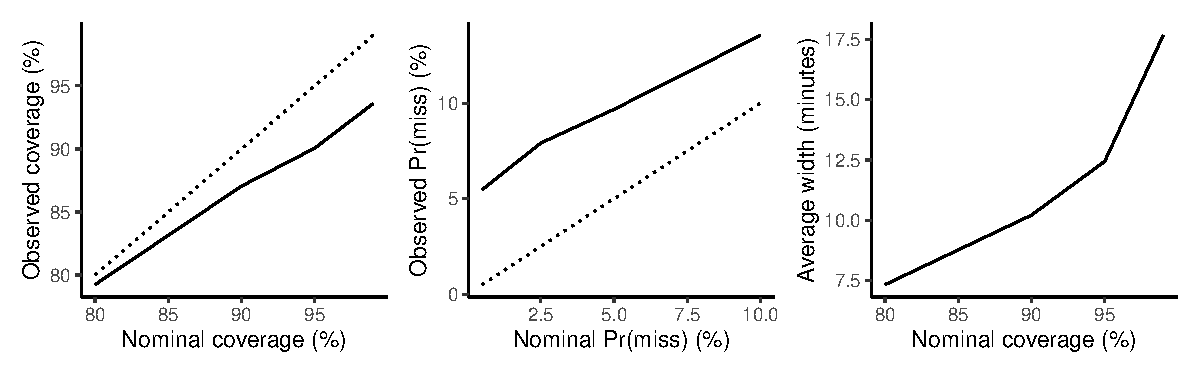
\includegraphics[width=\textwidth]{figure/eta_cis-1} 

}

\caption[ETA CIs]{ETA CIs}\label{fig:eta_cis}
\end{figure}


\end{knitrout}




We computed intervals for $\alpha \in \{0.1, 0.05, 0.1, 0.2\}$, and for each evaluated the observed coverage, the proportion of times that the bus arrived before the lower bound, and the average interval width (in minutes). \Cref{fig:eta_cis} shows that the observed coverage drops slightly as the interval width increases (smaller $\alpha$), and that the probability of the bus arriving before the lower bound is higher than expected, which could indicate that not enough uncertainty is being incorporated. Interval width increases rapidly with interval width, demonstrating the trade-off between reliability and usefulness.


We do not consider other variables---time until arrival, time of day, or stop sequence---as we did in the previous chapter, as the results will be much the same. However, if desired, such relationships could be explored in order to choose the best point or interval estimate under each situation.
